\documentclass[12pt]{article}

\usepackage[utf8]{inputenc}
\usepackage[T1]{fontenc}
\usepackage[brazilian]{babel}
\usepackage{geometry}
\usepackage{times}
\usepackage{graphicx}
\usepackage{url}
\usepackage{booktabs}
\usepackage{float}
\usepackage{hyperref}
\usepackage{longtable}
\usepackage[round]{natbib}
\usepackage{xcolor}
\usepackage{tikz}
\usetikzlibrary{arrows.meta,positioning,shapes.geometric}
\usepackage[ruled,vlined,linesnumbered,portuguese]{algorithm2e}

\geometry{a4paper,top=3.5cm,bottom=2.5cm,left=3.0cm,right=3.0cm}
\setlength{\parindent}{1.25cm}
\setlength{\parskip}{0pt}
\sloppy

\newenvironment{resumo}
{\begin{center}\textbf{Resumo}\end{center}\begin{quote}\small}
{\end{quote}}

\SetKwInput{KwEntrada}{Entrada}
\SetKwInput{KwSaida}{Saida}
\SetKw{KwProxima}{Na proxima execucao}

\title{Clusterizacao semantica e classificacao hibrida de noticias sobre operacoes da Policia Federal}
\author{Projeto NT PF}
\date{\today}

\begin{document}

\maketitle

\begin{abstract}
This paper describes a computational pipeline for transforming public news about Brazilian Federal Police operations into a structured analytical corpus. The method combines automated collection, textual extraction, hybrid classification with regular expressions and large language models, controlled summarization, semantic clustering, consensus analysis and continuous rule learning. Semantic clustering is used as an exploratory instrument, while hybrid classification produces auditable variables about crimes, modus operandi, affected sectors, actors and operational recurrence.
\end{abstract}

\begin{resumo}
Este artigo descreve uma metodologia computacional para transformar noticias publicas sobre operacoes da Policia Federal brasileira em uma base analitica estruturada. A proposta combina coleta automatizada, extracao textual, classificacao hibrida por expressoes regulares e modelos de linguagem, resumo controlado, clusterizacao semantica, consenso entre especificacoes e aprendizado continuo de regras. A estrategia separa duas finalidades: a clusterizacao semantica e usada como instrumento exploratorio para descobrir padroes no corpus; a classificacao hibrida e usada para produzir variaveis substantivas auditaveis sobre crimes, modus operandi, setor afetado, atores e recorrencia operacional. O resumo controlado e tratado como camada complementar, nao como substituto do texto integral.
\end{resumo}

\section{Introducao}

Noticias institucionais sobre operacoes policiais formam um corpus rico para observar recorrencias de crimes, modos de atuacao, territorios e formas de cooperacao estatal. Entretanto, esses textos tendem a ser heterogeneos: variam em extensao, estilo, nivel de detalhe, uso de tags, presenca de nomes de operacao e padrao narrativo. Essa heterogeneidade dificulta a construcao direta de categorias consistentes.

A metodologia proposta combina tres familias de tecnicas. Primeiro, utiliza representacoes vetoriais de texto e similaridade do cosseno para aproximar noticias semanticamente semelhantes, em linha com abordagens de embeddings e modelagem de topicos por agrupamento \citep{reimers2019sentencebert,grootendorst2022bertopic,angelov2020top2vec}. Segundo, aplica classificacao hibrida: regras deterministicas de alta confianca classificam casos claros, enquanto modelos de linguagem sao acionados para casos ambiguos ou nao capturados pelas regras \citep{gilardi2023chatgpt,rytting2023coding,heseltine2024llm,tornberg2025llm}. Terceiro, avalia a estabilidade dos agrupamentos por consenso entre especificacoes, inspirado na literatura de consenso de clusters \citep{monti2003consensus}.

\section{Dados}

O universo empirico e composto por noticias publicadas no portal publico da Policia Federal sobre operacoes. Cada noticia e representada como uma unidade documental. Para cada unidade, o pipeline preserva metadados objetivos e texto integral extraido em formato Markdown.

Os campos minimos previstos sao:

\begin{itemize}
    \item identificador ou link canonico da noticia;
    \item titulo e subtitulo;
    \item data de publicacao e, quando disponivel, data de atualizacao;
    \item URL de origem;
    \item texto integral extraido;
    \item tags institucionais;
    \item dateline, UF e municipio quando identificaveis;
    \item nome de operacao, quando explicitamente mencionado.
\end{itemize}

O pipeline tambem deve registrar controle de qualidade textual. Noticias vazias, incompletas, duplicadas ou sem corpo extraido suficiente devem receber flag propria, para que a analise principal consuma apenas registros validos.

\section{Pipeline metodologico}

A Figura~\ref{fig:fluxo-dados} apresenta o fluxo de dados da pipeline desde a extracao das noticias ate a classificacao, clusterizacao e publicacao dos artefatos analiticos. O desenho separa as camadas deterministicas, a camada semantica acionada por excecao e a etapa exploratoria de consenso.


\begin{figure}[H]
\centering
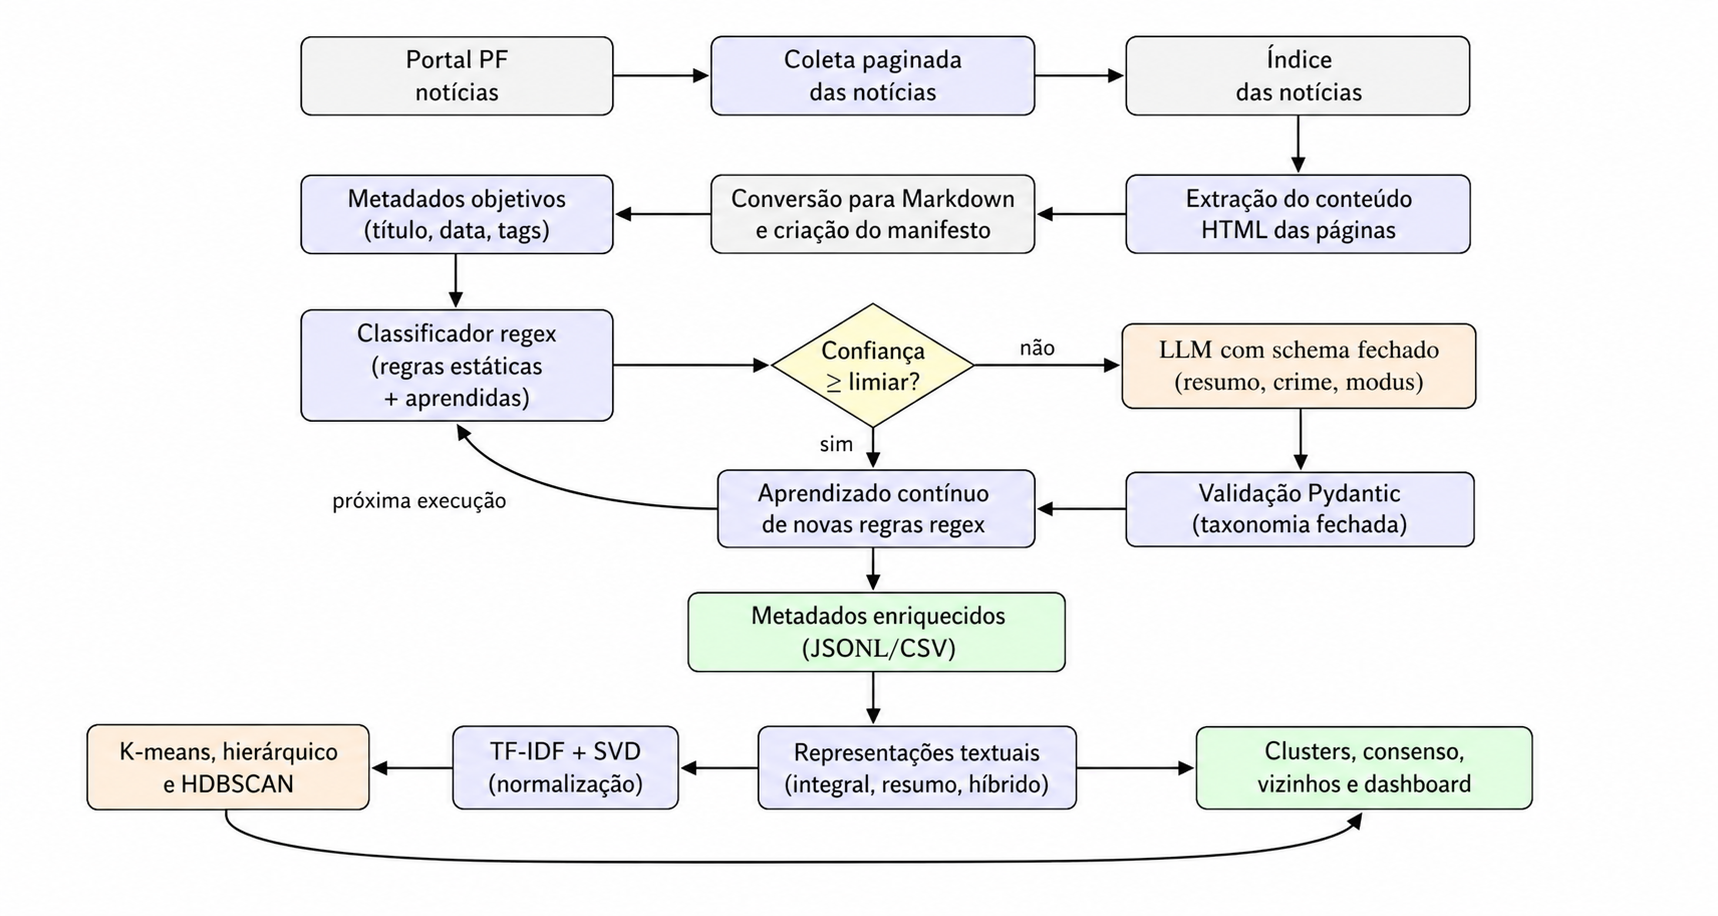
\includegraphics[width=\textwidth]{figures/pipeline.png}
\caption{Fluxo de dados da pipeline, da extracao das noticias a classificacao, aprendizado continuo, clusterizacao e geracao de artefatos.}
\label{fig:fluxo-dados}

\end{figure}

\begin{enumerate}
    \item Coleta da listagem paginada de noticias.
    \item Extracao do conteudo principal de cada pagina individual.
    \item Conversao do conteudo para Markdown e padronizacao dos metadados.
    \item Limpeza textual sem remover informacao substantiva.
    \item Classificacao por regras regex de alta confianca.
    \item Encaminhamento dos casos nao cobertos ou conflitantes para LLM.
    \item Geracao de resumo curto, resumo estruturado, evidencia textual, atores e setor afetado.
    \item Construcao de tres representacoes textuais: integral, resumida e hibrida.
    \item Clusterizacao semantica e recuperacao de vizinhos por similaridade do cosseno.
    \item Experimento de consenso entre especificacoes alternativas.
    \item Aprendizado continuo de regras regex a partir dos casos encaminhados a LLM.
    \item Producao da base final e dos artefatos analiticos.
\end{enumerate}

\section{Preparacao textual}

Cada noticia e convertida para texto limpo, preservando nomes de operacoes, orgaos, crimes mencionados, localidades, valores, mandados e outros sinais substantivos. Elementos repetitivos de pagina, menus, rodapes e links irrelevantes devem ser removidos. A geografia e tratada separadamente: termos geograficos podem ser removidos da representacao semantica para evitar que clusters sejam dominados por UF ou municipio, mas sao preservados como variaveis analiticas.

\section{Classificacao hibrida}

A classificacao final e concebida como um sistema em camadas. A primeira camada aplica expressoes regulares versionadas para padroes de alta confianca. Exemplos incluem mencoes diretas a lavagem de dinheiro, garimpo ilegal, pornografia infantil, fraude previdenciaria, descaminho, corrupcao e trafico de drogas.

Cada regra deve preservar:

\begin{itemize}
    \item classe atribuida;
    \item regra acionada;
    \item trecho que acionou a regra;
    \item nivel de confianca;
    \item versao da regra.
\end{itemize}

Casos nao capturados ou com sinais conflitantes sao encaminhados a uma LLM. A LLM nao recebe uma tarefa aberta; ela deve escolher exclusivamente entre categorias da taxonomia, retornar JSON valido e indicar evidencia textual curta. A saida estruturada inclui classe principal, classes secundarias, modus operandi, setor afetado, atores mencionados, resumo curto, resumo estruturado, confianca e flag de reprocessamento automatico. Portanto, o papel da LLM no projeto nao e substituir todo o classificador: ela funciona como camada semantica controlada, acionada quando a camada barata de regex nao resolve o caso, e como fonte de exemplos para o aprendizado continuo de novas regras.

\section{Resumo controlado como camada complementar}

O comentario metodologico que motivou esta atualizacao sugere que resumos curtos podem ajudar na clusterizacao semantica e na criacao de categorias. A proposta adotada e testar essa hipotese sem abandonar o texto integral.

Assim, o pipeline constroi tres representacoes:

\begin{description}
    \item[Texto integral] titulo, subtitulo e corpo normalizado. Serve para descoberta livre e exploratoria.
    \item[Texto resumido] titulo, subtitulo, resumo curto, resumo estruturado, evidencia, atores e setor afetado. Serve para reduzir heterogeneidade narrativa.
    \item[Texto hibrido] combina identidade canonica, crimes, modus, tags, resumo e texto integral. Serve como representacao principal do painel.
\end{description}

Essa decisao permite comparar se o resumo melhora estabilidade e interpretabilidade ou se perde informacao substantiva relevante. A expectativa e que os dois usos sejam complementares: o texto integral favorece descoberta; o resumo favorece padronizacao.

\section{Clusterizacao semantica}

Cada noticia e representada em um espaco vetorial. A implementacao atual usa TF-IDF, reducao por SVD e normalizacao, mantendo similaridade do cosseno como metrica de proximidade. A metodologia tambem e compatavel com embeddings neurais, como Sentence-BERT, ou modelos de topicos baseados em embeddings e agrupamento, como BERTopic e Top2Vec \citep{reimers2019sentencebert,grootendorst2022bertopic,angelov2020top2vec}.

A clusterizacao principal utiliza K-means em mini-lotes. O numero de clusters e escolhido por avaliacao de silhouette em uma grade de valores. Como alternativa metodologica, o experimento de consenso tambem aplica clusterizacao hierarquica e HDBSCAN sobre as representacoes integral, resumida e hibrida \citep{campello2013hdbscan}.

O HDBSCAN entra como apoio exploratorio, nao como classificacao final. Sua utilidade decorre de cinco propriedades: nao exige definir previamente o numero de clusters; permite marcar ruido e outliers; lida melhor com grupos de tamanhos diferentes; pode revelar subtemas densos dentro de categorias grandes, como corrupcao, crimes ambientais ou crimes contra criancas; e aumenta a robustez do consenso quando concorda com K-means e clusterizacao hierarquica. Por isso, o K-means permanece como cluster principal do painel, enquanto o HDBSCAN opera como diagnostico de estabilidade e descoberta de agrupamentos naturais.

\section{Consenso e estabilidade}

Como uma solucao unica de clusterizacao pode depender de algoritmo, parametros e representacao textual, a metodologia inclui um experimento de consenso. Para cada noticia, sao salvos os clusters obtidos em diferentes especificacoes. Em seguida, o pipeline calcula pares estaveis entre vizinhos semanticos: dois documentos formam um par estavel quando aparecem juntos em pelo menos 80\% das especificacoes validas.

Essa abordagem evita gravar uma matriz completa de coocorrencia para milhares de documentos e produz um artefato interpretavel: uma lista de pares robustos. Esses pares orientam a nomeacao automatica de clusters, o aprendizado de novas regras e a construcao incremental de categorias dentro da taxonomia existente.

\section{Taxonomia substantiva}

A taxonomia e organizada em multiplos niveis. O primeiro nivel cobre grandes areas, como corrupcao, lavagem de dinheiro, trafico de drogas e armas, crimes ambientais, crimes financeiros, fraudes previdenciarias, crimes ciberneticos, crimes eleitorais, fronteira e outros. O segundo nivel detalha tipos especificos de crime. O terceiro nivel descreve modus operandi, como empresa de fachada, uso de laranjas, contratos simulados, notas fiscais falsas, criptoativos, transporte aereo, transporte maritimo, servidores publicos envolvidos e documentos falsos.

Uma noticia pode receber multiplos rotulos. Portanto, a classificacao deve ser tratada como multilabel, e nao como atribuicao exclusiva de uma unica categoria.

\section{Aprendizado continuo}

A classificacao foi desenhada para nao depender de intervencao humana nessa etapa do processo. O ciclo de melhoria ocorre automaticamente. Primeiro, regras regex classificam os casos de alta confianca. Segundo, casos abaixo do limiar, conflitantes ou nao cobertos sao enviados para a LLM. Terceiro, a resposta da LLM e validada por schema e normalizada para a taxonomia permitida. Quarto, quando a LLM atribui rotulos com evidencia textual suficiente, o sistema tenta derivar padroes regex candidatos. Quinto, filtros automaticos removem padroes frageis, genericos, malformados ou sem evidencia lexical da classe atribuida.

As regras aprendidas sao gravadas em arquivo versionavel e entram na execucao seguinte do classificador. Dessa forma, a cobertura tende a aumentar ao longo das rodadas, enquanto a taxonomia permanece controlada. A LLM nao cria categorias livres; ela opera dentro de listas permitidas, e o aprendizado de regras e condicionado por evidencias extraidas do proprio texto.

\begin{algorithm}[ht]
\caption{Reducao de custo por aprendizado continuo de regras}
\label{alg:aprendizado-continuo}
\KwEntrada{Noticia em Markdown, regras regex estaticas, regras aprendidas e limiar de confianca.}
\KwSaida{Inferencia validada, fonte da classificacao e novas regras candidatas.}
\ForEach{noticia no corpus}{
    extrair metadados objetivos do Markdown\;
    aplicar o classificador regex com regras estaticas e aprendidas\;
    \eIf{a confianca do regex e maior ou igual ao limiar}{
        aceitar a inferencia regex\;
        registrar a fonte da classificacao como \texttt{regex}\;
        registrar custo de LLM igual a zero\;
    }{
        enviar a noticia para a LLM com schema fechado\;
        validar e normalizar a resposta com Pydantic\;
        registrar a fonte da classificacao como \texttt{llm}\;
        derivar regras regex candidatas a partir da inferencia e da evidencia textual\;
        remover regras frageis, genericas, malformadas ou sem evidencia lexical\;
        salvar as regras aprovadas no arquivo versionavel de regras aprendidas\;
    }
}
\KwProxima: carregar as regras aprendidas antes de chamar a LLM, aumentando a cobertura local por regex e reduzindo chamadas futuras ao modelo.
\end{algorithm}

\section{Artefatos esperados}

Ao final, cada noticia deve compor uma linha na base estruturada com campos como:

\begin{longtable}{ll}
\toprule
Campo & Descricao \\
\midrule
\endhead
link & URL ou identificador canonico da noticia \\
data & data normalizada de publicacao \\
uf, municipio & localidade extraida ou inferida \\
titulo & titulo original \\
cluster\_id & cluster exploratorio principal \\
cluster\_canonico & agrupamento guiado por identidade padronizada \\
classe\_principal & categoria substantiva principal \\
classes\_secundarias & categorias adicionais \\
crime\_investigado & crimes multilabel \\
modus\_operandi & modos de atuacao multilabel \\
setor\_afetado & setor ou politica publica afetada \\
atores\_mencionados & atores explicitamente citados \\
resumo\_curto & frase factual controlada \\
evidencia\_textual & trecho justificativo curto \\
metodo\_classificacao & regex, regex\_rescue ou LLM \\
regra\_acionada & regra deterministica, quando houver \\
confianca & confianca ou limiar aplicavel \\
precisa\_reprocessamento & flag de ambiguidade ou conflito para nova rodada automatica \\
\bottomrule
\end{longtable}

\section{Resultados da execucao local}

A pipeline foi reexecutada localmente em 08/05/2026 apos a incorporacao do HDBSCAN e a correcao do controle incremental por arquivo markdown. A etapa de metadados processou 8.048 arquivos markdown. Desse total, 7.884 foram resolvidos diretamente por regex e 164 exigiram chamada a LLM. Em termos operacionais, isso significa que aproximadamente 98\% dos arquivos foram classificados pela camada barata e deterministica, enquanto cerca de 2\% precisaram da camada semantica mais custosa.

O aprendizado continuo tambem foi acionado na execucao. Foram identificados 123 registros com sugestoes de aprendizado e 136 sugestoes de regra. A base consolidada de regras aprendidas passou a conter 18 grupos e 168 padroes. Esses numeros indicam o papel pratico da LLM no projeto: ela nao substitui o classificador principal, mas cobre casos nao resolvidos por regex e gera exemplos que podem reduzir chamadas futuras.

A etapa analitica produziu um corpus enriquecido com 8.055 noticias, apos remover 59 links duplicados do indice antes do merge. No corpus final, 7.891 noticias ficaram associadas a classificacao por regex e 164 a classificacao por LLM. A clusterizacao principal gerou 16 clusters por K-means, e a camada canonica produziu 38 grupos substantivos.

O experimento de consenso produziu 15.276 pares estaveis a partir de 9 especificacoes: K-means, hierarquico e HDBSCAN aplicados as representacoes integral, resumida e hibrida. O HDBSCAN marcou como ruido 5.662 noticias na representacao integral, 7.442 na resumida e 3.718 na hibrida. Esse comportamento confirma seu papel exploratorio: ele e mais rigoroso para formar grupos densos, ajuda a identificar outliers e subtemas, mas nao deve ser usado isoladamente como classificacao final.

\section{Exemplos de classificacao}

Para tornar a classificacao mais transparente, esta secao apresenta dois exemplos reais do corpus. O primeiro mostra um caso resolvido diretamente por regex, sem custo de LLM. A noticia ``PF combate exploracao ilegal de madeira e garimpo em terra indigena no Para'' acionou regras associadas a crimes ambientais, extracao ilegal de madeira e exploracao ilegal de recursos naturais. Como a confianca regex foi 0,95, acima do limiar operacional, a noticia foi classificada como \texttt{crimes\_ambientais}, com modus operandi \texttt{cooperacao\_interagencias} e \texttt{desarticulacao\_rede}. O resultado e auditavel porque os termos que acionaram a regra ficam registrados junto da inferencia.

O segundo exemplo mostra o papel complementar da LLM. A noticia ``PF desarticula comercio ilegal de medicamentos em Campo Grande/MS'' gerou sinais regex relevantes, como busca e apreensao, comercio ilegal e cumprimento de mandado, mas a confianca preliminar ficou em 0,74, abaixo do limiar. Nesse caso, a LLM foi acionada com schema fechado e retornou a identidade canonica \texttt{crime\_comercializacao\_medicamentos\_nao\_autorizados}, classificacao por crime, modus \texttt{busca\_apreensao} e \texttt{cumprimento\_mandado}, alem de resumo curto e evidencia textual. O ponto metodologico e que a LLM nao decide livremente toda a base: ela atua nos casos residuais e pode gerar evidencias para novas regras candidatas.

\section{Discussao}

A combinacao de clusterizacao semantica e classificacao hibrida equilibra descoberta e mensuracao. A clusterizacao explora padroes sem impor categorias previamente fechadas. A classificacao transforma esses padroes em variaveis auditaveis. O resumo controlado adiciona uma representacao padronizada, especialmente util quando os textos originais sao heterogeneos. O aprendizado continuo e o consenso entre especificacoes reduzem o risco de tratar agrupamentos instaveis ou inferencias incertas como resultado substantivo.

\section{Conclusao}

A metodologia proposta organiza um corpus de noticias de operacoes da Policia Federal em uma base estruturada, reprodutivel e auditavel. O ponto central e nao escolher entre texto integral, resumo, regex ou LLM, mas combinar essas camadas com funcoes distintas. Texto integral serve a exploracao; resumo controlado serve a padronizacao; regex oferece alta precisao em casos claros; LLM cobre ambiguidade; consenso mede estabilidade; aprendizado continuo amplia cobertura sem intervencao humana obrigatoria.

\bibliographystyle{apalike}
\bibliography{references}

\end{document}
